\documentclass[a4paper]{article}
%\documentclass[12pt,aps,pre,nofootinbib]{revtex4-1}
\usepackage[colorinlistoftodos,prependcaption,textsize=tiny]{todonotes}
\usepackage[english]{babel}
\usepackage[utf8x]{inputenc}
\usepackage{amsmath,amsfonts,amssymb,amsthm}
\usepackage{graphicx}
\usepackage{subfig}
\usepackage{hyperref}
\usepackage{color}
\usepackage{hyphenat}
\usepackage{natbib}
\usepackage{microtype}
\usepackage{mathpazo}
\usepackage{fancyhdr}
\usepackage{cleveref}
\usepackage{listings}

\makeatletter
\renewcommand*\env@matrix[1][\arraystretch]{%
  \edef\arraystretch{#1}%
  \hskip -\arraycolsep
  \let\@ifnextchar\new@ifnextchar
  \array{*\c@MaxMatrixCols c}}
\makeatother

\newcommand{\brho}{\boldsymbol \rho}
\newcommand{\bsigma}{\boldsymbol \sigma}
\newcommand{\btheta}{\boldsymbol \theta}
\newcommand{\bmu}{\boldsymbol \mu}
\newcommand{\bD}{\mathbf{D}}
\newcommand{\bA}{\mathbf{A}}
\newcommand{\bH}{\mathbf{H}}
\newcommand{\bL}{\mathbf{L}}
\newcommand{\Tr}[1]{\operatorname{Tr}\left\lbrack #1\right\rbrack}
\newcommand{\bE}[1]{\operatorname{\mathbb{E}}\left\lbrack #1\right\rbrack}
%\newcommand{\bE}[1]{\left\langle #1 \vert \btheta \right\rangle }
\renewcommand{\Im}[1]{\operatorname{Im}\left( #1\right)}
\newcommand{\pin}{p_{\textrm{in}}}
\newcommand{\pout}{p_{\textrm{out}}}
\newcommand{\bra}[1]{\left \langle #1 \right|}
\newcommand{\ket}[1]{\left | #1 \right \rangle}
\newcommand{\euler}{e}
\newcommand{\ramuno}{i}

\DeclareMathOperator\arctanh{arctanh}
\DeclareMathOperator\corr{corr}

\begin{document}
\title{Spectral entropies in correlation models of brain functional connectivty}
\author{Carlo Nicolini}
\date{\today}
\maketitle

\section{A simple model of correlation for brain fMRI}
Here we study a model of brain functional connectivity that tries to best reflect the properties of the Crossley full Fisher-transformed correlation matrix.
We constructed a benchmark correlation network by first choosing the number $n$ of time series, the membership vector $c_i$, defining the nodes within each community. The total number of communities is denoted by $|c|$.
For the membership vector I applied Louvain community detection method on the percolation thresholded Crossley matrix, obtaining a total of 6 communities of different sizes.
Then, we generated $|c_i|$ random and uncorrelated time series (with $T>n$) with values $\gamma_A(t)$ (where $1\le A\le c$) drawn independently from a normal distribution with zero mean and unit variance.
We created $|c_i|$ identical copies of the $A$-th time series, for all nodes in the community $c_i$.

To each of the resulting $n$ time series, each labeled by an index $i$, we added a local noise $\eta \beta_i(t)$ (a new normally distributed random variable with zero mean and $\eta$ variance, independent of all the other ones) and a global signal $\mu \alpha(t)$ an independent normally distributed random variable with zero mean and $\mu$ variance.
This resulted in a set $\{y_1,\dots,y_n\}$ of $n$ time series with values:
\begin{equation}
y_i(t)= \gamma_A(t) + \nu\cdot \beta_i(t) + \mu\cdot \alpha(t) \quad i\in A, \quad A=1,\ldots,c
\label{eq:bench}
\end{equation}
The time series $\{y_1,\dots,y_n\}$ are further \emph{standardized} to obtain a final set $\{x_1,\dots,x_n\}$ of $n$ time series, each with zero mean and unit variance.
The obtained z-transformed correlation matrix of the factor model can be written as:
\begin{equation}
B_{ij} = \arctanh\left( \corr(X_i, X_j) \right)
\end{equation}
and is the basis of our analysis, as it becomes a benchmark network to test the value of the spectral entropies appproach.
By appropriately tuning the local noise and global noise parameters, it is possible to best reflect the properties of the Crossley network.
I have shown that the histogram of the edge weights of the Fisher transformed correlation matrix from these benchmark networks, reflects pretty well the distribution of the Fisher z-values of the original Crossley matrix, when the model parameters are tuned to $T=200$ time points, local noise $\eta=2.5$, global noise $\mu=1.5$, soft-threshold coefficient $\gamma=1$ and multiplicative factor $q=0.8$
\begin{figure}
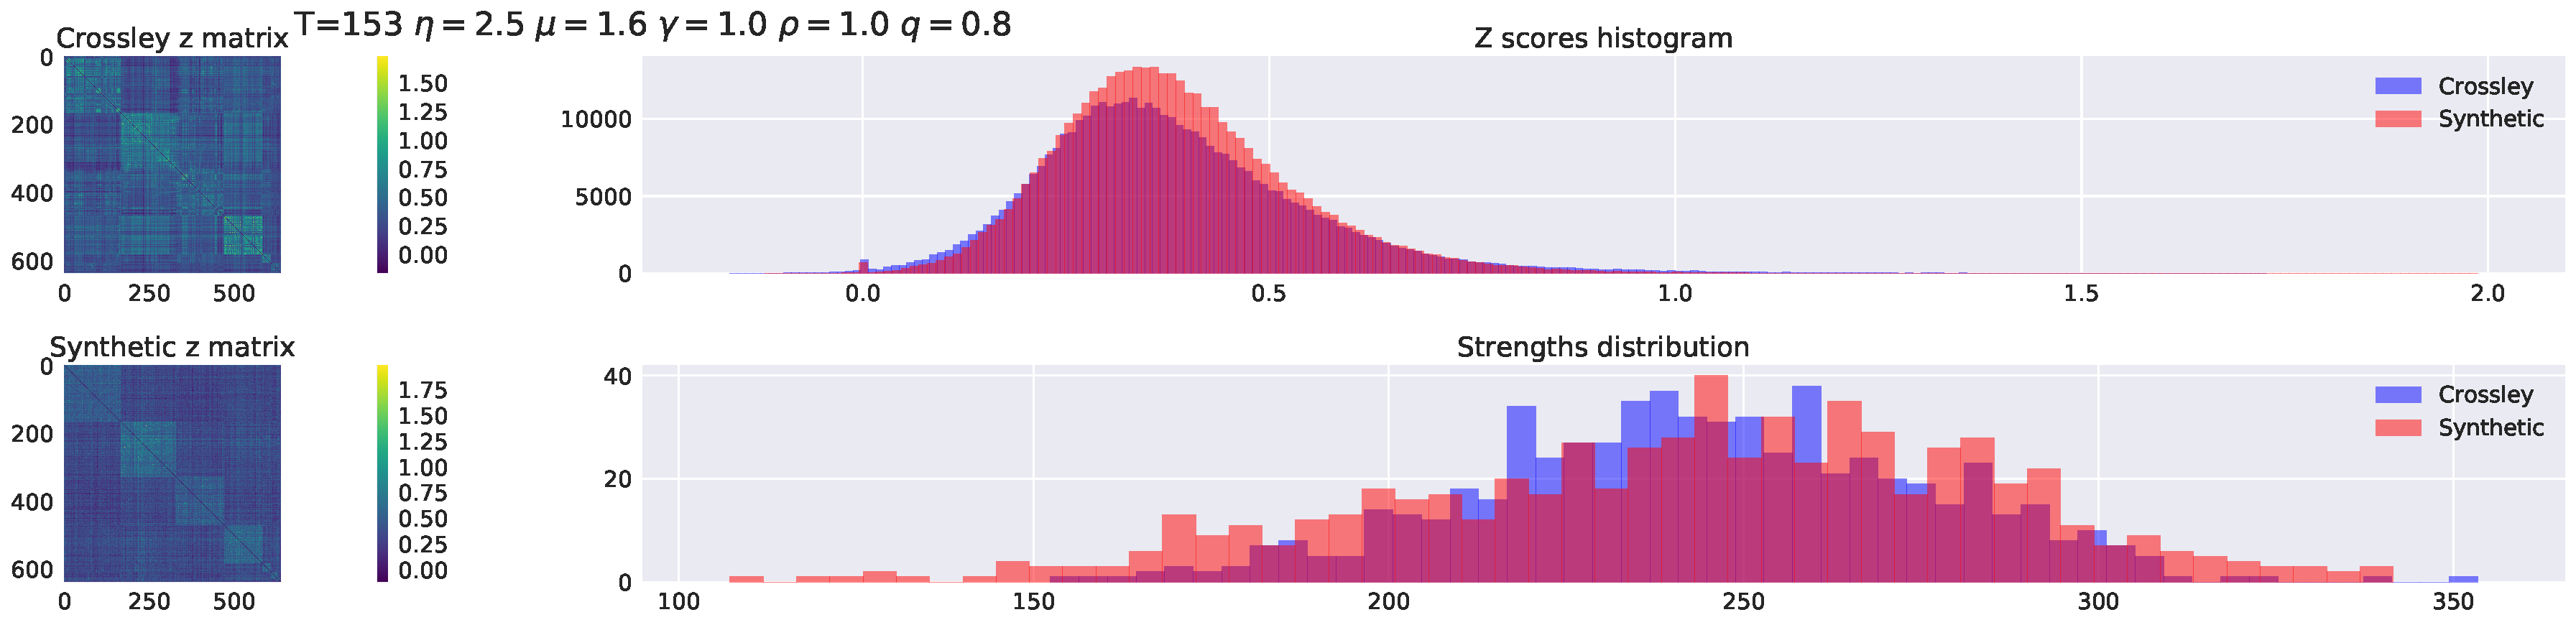
\includegraphics[width=1.0\textwidth]{../crossley_vs_synthetic.pdf}
\caption{Comparison between the crossley z matrix and the synthetic one, with $T=200$ time points, local noise $\eta=2.5$, global noise $\mu=1.5$, soft-threshold coefficient $\gamma=1$ and multiplicative factor $q=0.8$.}
\label{fig:benchmark_network}
\end{figure}

These parameters make the factor model simple enough to study in the settings of the spectral entropies method. In Figure~\ref{fig:benchmark_network} a realization of the model is shown that reflects with good confidence the Crossley network.

\section{Spectral entropies as function of the global noise}
The effect of the global noise parameter is to introduce correlation between all the time-series, resulting in a shift in the global z-score and effects on the spectral entropy. 
Here we try to hypothesize the following phenomenon. As an effect of global correlation increase, with increasing edge weights, the diffusion properties of the network are changing. In particular, with higher ``flux'' on the edges, the diffusion is faster, hence higher entropy is reached at smaller $\beta$.

\begin{figure}
\includegraphics[width=1.0\textwidth]{../spectral_entropy_synthetic_global_noise.pdf}
\caption{Increase in the global noise. The increase of the intermodule links weights, modifies the spectral entropy, inducing lower entropy at all scales.}
\label{fig:benchmark_network}
\end{figure}
The hypothesis seems to be confirmed by experimental data.

\newpage
\subsection{Edge removal effect}
In this experiment we studied the effect on the transition with respect to $\beta$ of the spectral entropy as a function of the percentage of the edges removed from a fully connected graph.
The close a network becomes to the fully connected uniform topology, the steeper is the entropy difference in a small range of $\beta$, a quantity that can be measured by the width of the peak in the derivative of the entropy with respect to $\beta$ as shown in Figure~\ref{fig:beta_deriv_clique_removal}:
\begin{figure}[htb]
\centering
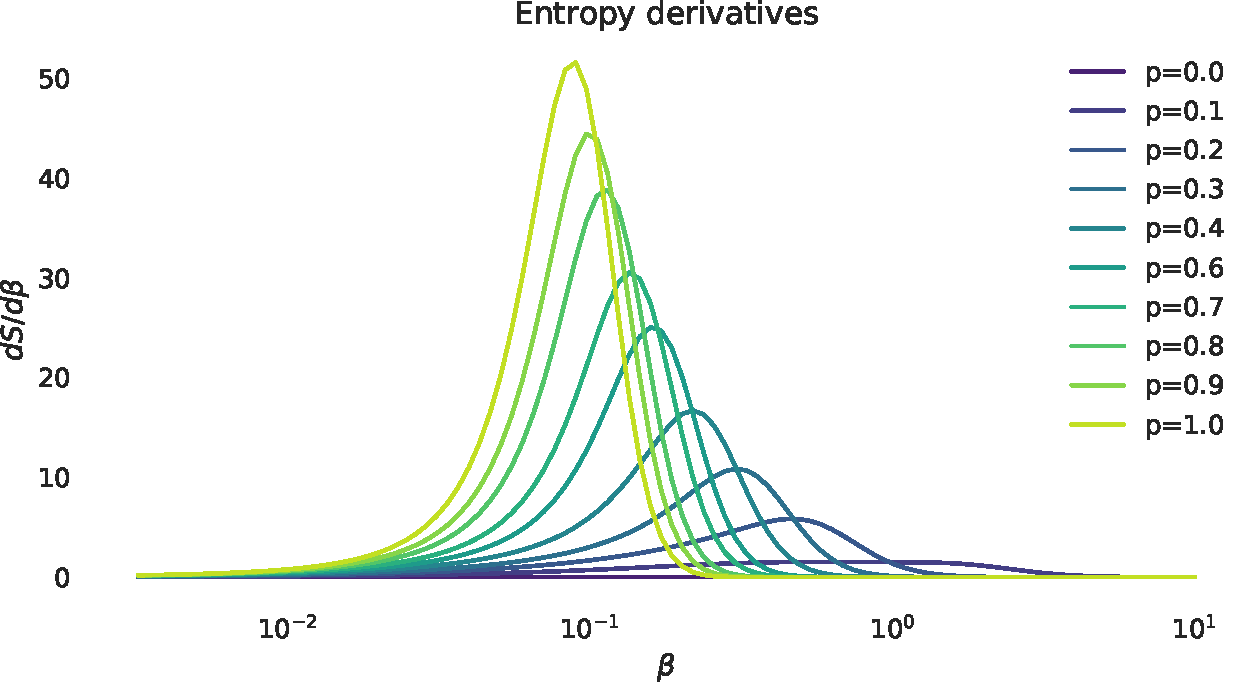
\includegraphics[width=0.8\textwidth]{entropy_derivative_er.pdf}
\caption{Effect of link removal on the FWHM of the quantity $dS/d\beta$. At full densities (yellow curves) the entropy derivative is steeper, hence the peak is higher. Empty networks have a slower rate of diffusion. }
\label{fig:beta_deriv_clique_removal}
\end{figure}

We replicate the same experiment in the case of weighted correlation networks

\newpage
\section{A push-pull effect on spectral entropies}
A nice interpretation of the curves of spectral entropies are the following.
We have observed that increasing the global number of links, for example by multiplying the whole network by a factor then, returns that same entropy for a $\beta$ factor of the same inverse factor.
For example, if for a network $\bA^*$ and $\beta^*$ we have entropy $S(\bA^*, \beta^*)$, we can get the same entropy if we multiply (or divide) the network by a constant factor $\gamma$ and divide (or multiply) the same network for the same factor: $S(\bA^*, \beta^*) = S(\gamma \bA^*, \beta^* \gamma^{-1})$. This effect is due to the multiplicative effect over every eigenvalue.

\begin{figure}[htb]
\centering
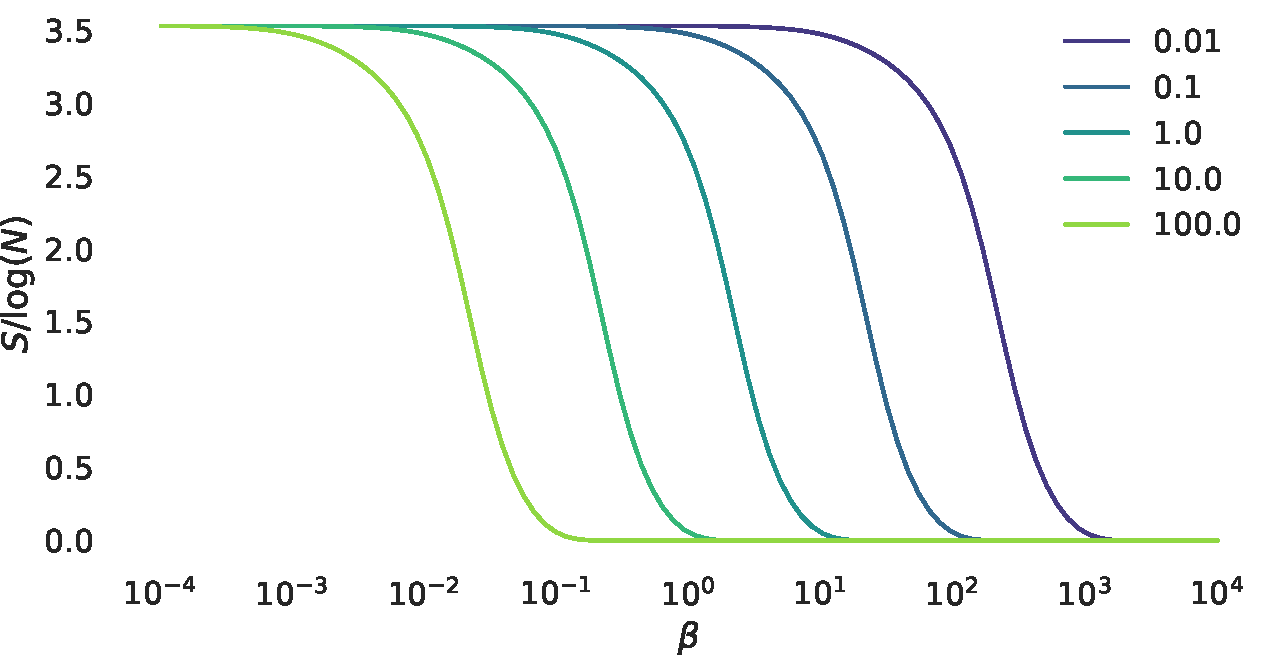
\includegraphics[width=0.8\textwidth]{multiplier_effect.pdf}
\caption{Effect of global multiplication of link weight in the spectral entropy curves for the karate club graph. On x-axis is $\beta$. An increase in the multiplicative factor has the effect of shifting the entropy curves to the left, in areas of smaller $\beta$.}
\label{fig:entropy_curves_unnormalized}
\end{figure}
This overall multiplication corresponds to increasing the flow over the links of the network by the same factor, or in visual terms, by shifting the entropy.
With this in mind, we can try to increase the weight of all links in a subset of nodes of a complete graph, an operation that should look similar to an artificial increase of the modularity of a subset of nodes.

\subsection{Comparison of different networks}
This observation makes evident that in order to compare two networks with a different number of nodes, in terms of their spectral entropies, one has to normalize the adjacency matrix by the total number of links. With this normalization, the curves in~\ref{fig:entropy_curves_unnormalized} are translated within a smaller range.

\begin{figure}[htb]
\centering
%\includegraphics[width=0.8\textwidth]{}
\caption{xxx}
\label{fig:entropy_curves_normalized}
\end{figure}

\begin{figure}

\begin{tikzpicture}[domain=0:4]
\filldraw [fill=blue] plot[id=f1,domain=-3:-2] function {exp(-x*x/2)}
            -- (-2,0) -- (-3,0) -- cycle;
\end{tikzpicture}

\end{figure}
\end{document}
